\section{The Language}\label{sec:lang}
%
This section presents an overview of the conceptual modeling language.
The concrete syntax will be presented using examples.
The abstract syntax will be presented in more detail in the next subsections; each one focusing on a key concept of the language's metamodel. (The appendix \ref{sec:spec} provides a formal description of the concrete syntax, along with its mapping to the abstract syntax.)

Before exploring the abstract syntax, a concrete example is displayed in figure \ref{fig:store} and commented below:

\begin{figure}
\verbatimfont{\small}
\begin{verbatim}
concept BookStore
{
    books: Book+;
    customers: Customer*;
    orders: Order*;
    /goldCustomers = customers | select totalSales > 1000;
    /orderedBooks = orders.items.book;
}

concept Book
{
    title: String;
    price: Decimal;
    quantity: Integer = 0;
}

concept Customer
{
    orders: Order*;
    /totalSales = orders | collect result += total;
}

concept Order
{
    customer: Customer;
    total: Decimal;
}

association CustomerOrder
{
    Order.customer: Customer;
    Customer.orders: Order*;
}
\end{verbatim}
\caption{The example above is adapted to CML from the fictional Livir bookstore, which is presented as a case study in Wazlawick \cite{wazlawick}.}
\label{fig:store}
\end{figure}


The model specified by the example above will be parsed and instantiated by the CML compiler into the following abstract syntax tree:

\label{fig:ast}
\begin{figure}
\centering
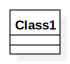
\includegraphics{language/main}
\caption{This is the caption of the figure displaying a white eagle and
a white horse on a snow field}
\end{figure}
